\documentclass{article}
\usepackage[utf8]{inputenc}
\usepackage[T1]{fontenc}
\usepackage[polish]{babel}
\usepackage{graphicx}
\usepackage{pdfpages}
\usepackage{minted}
\usepackage{diagbox}
\usepackage{subfig}
\usepackage{caption}
\usepackage{multirow}
\usepackage[a4paper,top=2cm, bottom=2cm]{geometry}
\renewcommand{\contentsname}{Spis treści}


\title{Implementacja oraz badanie transmisji w systemie ARQ}

\author{Leszek Błażewski, 241264 \\ \\Karol Noga, 241259 \\ \\Tomasz Dyśko, 241321}

\date{Semestr letni 2018/2019}

\begin{document}
\maketitle
\thispagestyle{empty}
\clearpage
\setcounter{page}{1}
\tableofcontents
\newpage{}

\section{Założenia projektowe}

Głównym celem projektu, była implementacja systemu kontroli błędów \textit{ARQ} - Automatic Repeat reQuest, poznanego podczas wykładów w poprzednim semestrze. Dodatkowo należało przeprowadzić symulację zaimplementowanego systemu oraz badania transmisji w których wykorzystano zbudowany model. Ostatnim etapem realizowanego projektu była analiza otrzymanych danych przy użyciu narzędzi statystycznych, które pozwoliły na graficzną reprezentację badanego zagadnienia oraz wyznaczenie parametrów potrzebnych do wyciągnięcia odpowiednich wniosków, dotyczących danych algorytmów.

\subsection{Wymagania systemu} \label{Wymagania}

Program powinien symulować przesył danych w kanale, pozwalać na modyfikację konkretnych wartości dotyczących przesyłanych sygnałów oraz wyznaczanie statystyk dotyczących konkretnych parametrów. Na podstawie otrzymanych danych wyznaczony zostanie najbardziej optymalny oraz skuteczny protokół pozwalający osiągnąć największą skuteczność dla zadanych parametrów.

Poniżej zamieszczono pełną listę wymagań, które powinna spełniać końcowa aplikacja.

\begin{itemize}
    \item Możliwość przeprowadzanie transmisji z wykorzystaniem modelu \textit{ARQ}.
    \item Implementacja dwóch kanałów transmisji.
    \item Możliwość przeprowadzenia badań dla różnych protokołów wykorzystywanych przez system \textit{ARQ}.
    \item Zastosowanie różnych sposobów kontroli błędów dla badanego modelu.
    \item Generowanie wykresów pozwalających na graficzną reprezentację otrzymanych danych.
\end{itemize}

\section{Technologie i narzędzia}

Rozdział ten traktuje o argumentach, które skłoniły nas do wyboru danego języka oraz zawiera krótki opis narzędzi i technologi, które wykorzystaliśmy w projekcie.

Cały projekt wraz z dokumentacją dostępny jest w publicznym repozytorium, które dostępne jest pod poniższym linkiem:

\begin{center}
\textbf{https://github.com/LeszekBlazewski/NiDUC}
\end{center}{}

Zdecydowaliśmy się zrealizować całą aplikację w środowisku \textit{MATLAB}, ponieważ oferuje ono szeroki wachlarz wbudowanych funkcji, które pozwoliły nam w prosty i szybki sposób zrealizować budowę całego modelu. Dodatkowym atutem była duża liczba dostępnych pakietów statystycznych, które również znaczenie uprościły cały proces analizy otrzymanych danych. Ostatnim czynnikiem, który zadecydował o wyborze powyższego środowiska była znajomość podstawowych funkcji oferowanych przez język, które poznaliśmy na poprzednich semestrach.

Cały tworzony kod przechowywany był w repozytorium umieszczonym w serwisie Github, dzięki czemu na bieżąco mogliśmy sprawdzać poprawność  kolejnych implementacji oraz w razie potrzeby, przywracać poprzednie wersje aplikacji.

\section{Implementacja}
Rozdział ten zawiera dokładne informacje dotyczące zaimplementowanych funkcji wraz z wycinkami kodu, które wymagają komentarza oraz realizują kluczowe funkcje, które zdefiniowane zostały w wymaganiach budowanego systemu. Kod źródłowy również zawiera komentarze, które tłumaczą sposób rozwiązania danego problemu i opisują wykorzystanie poszczególnych funkcji wbudowanych, które wykorzystane zostały do osiągnięcia danego celu.

\newpage

\subsection{Model systemu ARQ}

Postanowiliśmy wykorzystać algorytm \textit{stop and wait}, ponieważ jest on prostszy w implementacji od rozwiązania \textit{go back N} i w przypadku analizy jedynie wykrywania błędów bez ich korekcji dostarcza wszystkich potrzebnych danych do analizy.

Zasadniczy schemat działania algorytmu przedstawiony został na poniższym diagramie.


\begin{figure}[h!]
    \centering
    \includegraphics[width=\textwidth]{ARQ.png}
    \caption{Schemat działania systemu ARQ}
    \label{fig:StopAndWait}
\end{figure}

Na podstawie powyższego diagramu dokonano implementacji w języku \textit{matlab}. Całość zrealizowana została jako pętla, która w każdym swoim obiegu wykonuje sekwencję przedstawioną na powyższym rysunku.

Poniżej zamieszczono skrypt, odpowiedzialny za symulacje modelu \textit{ARQ}. Funkcja w zależności od przekazanych parametrów, realizuje odpowiedni proces kodowania i dekodowania, które omówione zostały w sekcji \ref{Kodowania}.

\newpage

\begin{minted}[fontsize=\small]{Matlab}
% ------------STOP AND WAIT-----------

function[operationCounter,decodedData]=ArqStopAndWait(data,probabilityOfError,canalName,codingProtocol)

operationCounter = 0;
[m,n] = size(data);
decodedData = zeros(m,n);
i = 1;

while (i <= m)
    % encode data
    switch codingProtocol
        case 'P2F5'
            encodedData = twoFromFiveCoding(data(i,:));
        case 'CRC'
            encodedData = crc16Coding(data(i,:));
        case 'PB'
            encodedData = parityBitCoding(data(i,:));     
    end
    
    % send through channel
    switch canalName
        case 'BSC'
            dataAfterTransmission = channelBSC(encodedData,probabilityOfError);
            
        case 'REC'
            dataAfterTransmission = channelREC(encodedData,probabilityOfError);
    end   
    
    % decode the data
    switch codingProtocol
        case 'P2F5'
            [decodedpacket,correct] = twoFromFiveDecoding(dataAfterTransmission);
        case 'CRC'
            [decodedpacket,error] = crc16Decoding(dataAfterTransmission);
            correct = ~error;
        case 'PB'
            [decodedpacket,correct] = parityBitDecoding(dataAfterTransmission);     
    end
    decodedData(i,:) = decodedpacket;
    
    % check if error occured
    if (correct)
        i=i+1;
    end
    operationCounter = operationCounter + 1;
end
end
\end{minted}

\subsection{Kanały transmisji}

W poniższym rozdziale opisano sposób realizacji dwóch kanałów telekomunikacyjnych, przez które przesyłane były pakiety. Każdy z kanałów odpowiedzialny był za wprowadzanie szumów do przesyłanych sygnałów, zmieniając losowe bity w przypadkowo wybranych pakietach. Kanały symulują dwa odmienne media transmisyjne, które różnią się od siebie sposobem wyboru pakietu w którym przekłamany zostanie bit.

\subsubsection{Binary symmetric channel}

Kanał \textit{BSC} jest powszechnie wykorzystywany w telekomunikacji z powodu łatwości w analizie oraz realnej symulacji losowych szumów występujących podczas każdej transmisji. Alfabet wejściowy i wyjściowy kanału są identyczne i wyrażają się w postaci \{0,1\} co oznacza, że jedynymi wartościami jakie można przesyłać przez kanał są ciągi $0$ i $1$. Cechą charakterystyczną kanału jest zmiana bitu na przeciwny z zadanym prawdopodobieństwem \textit{p}.

W symulatorze kanał został zaimplementowany z wykorzystaniem wbudowanej funkcji \textit{BSC} środowiska \textit{Matlab}.

\begin{minted}{Matlab}
%{
Function simulates the binary symmetric channel
parameters:
data - matrix of 0 and 1 which will be transported
probability - probablity of the error rate
returns:
matrix which contains data after the transmission through the canal
%}

function [ corruptedData ] = channelBSC( data, probability )

    corruptedData = bsc(data, probability);
end
\end{minted}

\subsubsection{Random error channel}

Jako drugi model kanału telekomunikacyjnego, postanowiliśmy wykorzystać własną implementację. Kanał symuluje ciągłe lekkie zaszumienie łącza wprowadzając błędy z małym prawdopodobieństwem, natomiast w losowych momentach występuje skok prawdopodobieństwa i przekłamaniu ulega większa liczba bitów. Kanał może być odwzorowaniem, losowych skoków napięcia występujących w medium transmisyjnym.

Poniżej zamieszczono kod funkcji odpowiedzialnych za generowanie błędów oraz realizację całego kanału.

\begin{minted}{Matlab}
%{
Function simulates continuous small changes and random peaks (e.g. voltage)
parameters:
data - matrix of 0 and 1 which will be transported
probability - probablity of the error rate
returns:
matrix which contains data after the transmission through the channel
%}
function [ corruptedData ] = channelREC( data, peakErrorProbability )
[ m, n ] = size(data);
corruptedData = zeros(m,n);
for i=1:m
    for j=1:n
        corruptedData(i,j) = data(i,j) + generateError(peakErrorProbability);
        if (corruptedData(i,j) >= 0.5)
            corruptedData(i,j) = 1;
        else
            corruptedData(i,j) = 0;
        end
    end
end
end

function [ error ] = generateError( peakErrorProbability )
error = 0.24 * randn();
if (peakErrorProbability >= rand())
    if (0.5 < rand)
        error = error + 0.5 + rand();
    else
        error = error - 0.5 - rand();
    end
end
end
\end{minted}

\subsection{Algorytmy detekcji błędów}  \label{Kodowania}

Głównym celem projektu była analiza możliwości systemu ARQ w zależności od stosowanego sposobu kodowania przesyłanych pakietów oraz ich rozmiaru. W celu przeprowadzenia odpowiednich badań, zaimplementowaliśmy trzy różne kodowania. Każde z zaproponowanych kodowań pozwala na detekcje błędów, natomiast kod \textit{CRC}, pozwala również na jego korekcję. Nie wykorzystaliśmy możliwości korekcji błędów, ponieważ badania oparte były wyłącznie na ilości błędów popełnianych dla danych kodowań.

\subsubsection{Cyclic redundancy check 16 bit}

Pierwszym z zaimplementowanych kodowań była szesnastobitowa wersja kodu \textit{CRC} w standardzie \textit{IBM/ANSI}. Dla tego standardu algorytm wykorzystuje wielomian $x^{16}+x^{15}+x^2+1$. Do implementacji wykorzystaliśmy wbudowaną funkcję, dostępną w środowisku \textit{Matlab}, dzięki czemu mieliśmy pewność co do poprawności przyjętej implementacji. Funkcja dodaje narzut równy 16 bitom, które stanowią sumę kontrolną przesyłanych danych. Dodawana suma jest wynikiem operacji \textit{XOR} pomiędzy bitami dzielnika (wielomianu dla danego kodu \textit{CRC} i odpowiednimi bitami ciągu danych, uwzględniając dopisane 16 bitów, wymaganych do poprawnego wytworzenia dodawanego narzutu.

\vspace{2mm}
\noindent
Poniżej zamieszczono implementację funkcji odpowiedzialnej za zakodowanie danych z wykorzystaniem wyżej opisanego algorytmu.

\begin{minted}{Matlab}
%{
    Function codes the given data with crc16 protocol.
    Parameters:
    data - matrix of zeroes and ones to encode
    returns:
    matrix with encoded data, where each row contains coded data with it's
    reminder
%}
function [codedData] = crc16Coding(data)
gen = comm.CRCGenerator([16 15 2 0],'ChecksumsPerFrame',1); % generator of checksum
[n,m] = size(data); % get number of rows (n) and number of columns (m)
codedData = zeros(n,m+16);% empty matrix for storing coded data, when using crc 16 
                          % protocol there are additional 16 columns added.

for x=1:n
    msg = data(x,:).'; % get row and transpose it because generator requires it
    codedData(x,:) = step(gen,msg).'; % uses generator to encode provided data and  
                                      % transpose it back to fit matrix
end
end
\end{minted}

Dekodowanie po otrzymaniu danych działa w analogiczny sposób. Po odkodowaniu operacją \textit{XOR} następuje sprawdzenie warunku, czy ostatnie 16 bitów odkodowanego wektora są równe 16 bitom wektora zakodowanego. Funkcja zwraca wektor z odkodowanymi danymi parametr, który zawiera informację o tym czy błąd wystąpił po zdekodowaniu danych. Jeśli zmieniony zostanie jeden z bitów w wiadomości, to suma sprawdzająca po odkodowaniu nie będzie równa zakodowanej i funkcja zwróci odpowiednią informację.

\vspace{2mm}
\noindent
Poniżej zamieszczono implementację funkcji odpowiedzialnej za zakodowanie danych z wykorzystaniem wyżej opisanego algorytmu.

\newpage

\begin{minted}{Matlab}
%{
    Function decodes the encoded parameter by crc16 protocol.
    Parameters:
    encodedData - horizontal vector which contains data encoded by crc 16
    returns:
    decodedData - horziontal vector which contains decoded data
    error - error which indicates whether any bit was corrupted during
    transmission ( in frame we are currently running one frame)
%}
function [decodedData, error] = crc16Decoding(encodedpacket)
encodedpacket = encodedpacket.';    %transpose the given  vector
detect = comm.CRCDetector([16 15 2 0],'ChecksumsPerFrame',1);   % create detector for CRC16
[decodedData, error] = step(detect,encodedpacket); % decode the given parameter
decodedData = decodedData.';
end
\end{minted}

\subsubsection{Two-out-of-five code}

Detekcyjny kod 2 z 5 polega na zakodowaniu każdego z wysyłanych bitów na 5 pozycjach. Dla $0$ są to $11000$, zaś dla $1$ wynoszą one odpowiednio $10100$. Założenie tego kodu opiera się na prostej tezie, iż istnieje mniejsze prawdopodobieństwo przekłamania $5$ bitów, niż jednego. Na 5 bitów w których kodowany jest jeden znak, występują 2 jedynki, jest to zatem kod stałowagowy. Minimalna odległość \textit{Hamming} dla zaprezentowanego kodu wynosi $2$.



\vspace{2mm}
\noindent
Poniżej zamieszczono implementację funkcji odpowiedzialnej za zakodowanie danych przy użyciu kodowania dwa z pięciu.

\begin{minted}{Matlab}
%{
Function codes the fiven data with the 2 from 5 protocol.
parameters:
data - matrix containing data which should be sent via the canal.
codedData - matrix which contains each bit coded in 2 from 5 protocol
%}

function [codedData] = twoFromFiveCoding( data )
[m, n] = size(data);
codedData = zeros(m, n*5);

for i = 1:m
    for j = 1:n
        x = 5*(j-1) + 1;
        if data(i,j) == 0
            codedData(i, x:x+4) = [1, 1 , 0, 0, 0];
        else
            codedData(i, x:x+4) = [1, 0 , 1, 0, 0];
        end
    end
end 
end
\end{minted}

\newpage

Dekodowanie polega na pobieraniu danych w paczkach po 5 bitów z otrzymanej wiadomości, a następnie należy porównać znaleziony ciągu z ustalonymi ciągami do kodowania zera i jedynki oraz  zapisać odpowiednią wartość do wektora przechowującego zdekodowane dane. Jeśli wynik porównania będzie fałszywy wiemy, że dany bit został przekłamany i dokonać należy retransmisji.

\begin{minted}{Matlab}
%{
Function decodes the given data vector in which data is coded in 2 from 5 protocol.
parameters:
receivedPacket - vector of size n which contains data coded with 2 from 5 protocol
returns:
uncodedData - vector of size n/5+1 with uncoded data. First bit in decoded vector
informs whether coded data was corrupted durning transmission.
isReceived - specifies whether packet given in parameter was corrupted
%}
function [uncodedData,IsReceived] = twoFromFiveDecoding( receivedPacket )
[~, n] = size(receivedPacket);
numberOfBits= n/5;
uncodedData = zeros(1, numberOfBits);
IsReceived = true;
codedOne = [1 0 1 0 0];
codedZero = [1 1 0 0 0];

for i=1:numberOfBits
    range = [(5*(i-1))+1 (5*i)];
    codedBit = receivedPacket(1,range(1):range(2));
    if isequal(codedBit, codedZero)
       uncodedData(i) = 0; 
    elseif isequal(codedBit, codedOne)
       uncodedData(i) = 1;
    else
       uncodedData(i) = 1;
       IsReceived = false;
    end
end    
end
\end{minted} 

\subsubsection{Parity bit}

Ostatnim z zaimplementowanych kodów, pozwalających na detekcję błędu jest proces dodawania bitu parzystości dla przesyłanego sygnału. Jest to jedna z najprostszych metod kontroli błędów, lecz jest ona obarczona dużym błędem i charakteryzuje się dużą zawodnością.
Na koniec wiadomości zostaje dodany bit parzystości, obliczany jako suma logiczna wszystkich „jedynek” występujących w przesyłanym sygnale.

\vspace{2mm}
\noindent
Poniżej zamieszczono funkcję odpowiedzialną, za wyznaczenie bitu parzystości dla danego wektora danych.

\newpage

\begin{minted}{Matlab}
%{
Function codes the given data matrix with pairity bit protocol.
Adds 0 or 1 based on the number of 1's in the matix.
parameters:
data - matrix with data which should be send
returns:
codedData - matrix with one addition column, representing the pairity
of data.
%}
function [codedData] = parityBitCoding( data )
%   kodowanie/kontrola bledow za pomoca bitu parzystosci

  [m,n] = size(data);
  codedData = zeros(m, n+1);
  for i = 1:m
      codedData(i,1:n) = data(i,1:n);
      codedData(i,n+1) = mod(sum(data(i,1:n)),2);
  end
end
\end{minted}

 Dekodowanie polega na odcięciu ostatniego bitu z wiadomości, następnie przeliczeniu bitu parzystości dla otrzymanej w ten sposób wiadomości i porównanie wyników. Metoda ta jest zawodna, gdyż jeśli zamienione zostaną dwa lub dowolna inna parzysta ilość bitów, algorytm nie będzie wstanie wykryć przekłamania. 
 
\begin{minted}{Matlab}
%{
Decodes the given data in parameter, byc calculating the sum of one's in
the packet.
parameters:
receivedPacked - packet which contains data, after transmission.
returns:
IsReceived - test whether the bit was correctly received
uncodedData - data without the pairity bit
%}
function [uncodedData,IsReceived] = parityBitDecoding( receivedPacket )
parityBit=receivedPacket(end);
receivedData=receivedPacket(1:end-1);
parityTest = mod(sum(receivedData),2);
if parityTest==parityBit
    IsReceived = true;
else
    IsReceived = false;
end
uncodedData=receivedData;

end
\end{minted}

\newpage

\section{Plan eksperymentu}

Głównym celem projektu była analiza zaimplementowanego modelu \textit{ARQ} oraz kodowań służących do wykrycia błędów podczas transmisji.

Celem naszych badań było wyznaczanie parametrów, które pozwolą porównać zaimplementowane kodowania oraz pokażą znaczące różnice pomiędzy algorytmami. Podczas wszystkich symulacji w różnych kanałach telekomunikacyjnych dla każdego z algorytmów detekcji błędów wyznaczyliśmy poniższą listę parametrów:

\begin{itemize}
    \item Liczbę błędnie przesłanych pakietów.
    \item Średnią liczbę błędnych pakietów.
    \item Odchylenie standardowe zestawu danych.
    \item Medianę zestawu danych.
    \item Wartość minimalną oraz maksymalną.
    \item Rozstęp międzykwartylowy.
    \item Ilość retransmisji przypadających na jeden pakiet.
    \item Narzut w postaci liczby nadmiarowych bitów wynikający z przyjętego kodowania.
\end{itemize}

Podczas każdej z symulacji przyjęliśmy stałą liczbę pakietów wynoszącą 10. W sprawozdaniu zamieszczono odpowiednie parametry statystyczne, wyznaczone na podstawie wygenerowanego zestawu danych podczas symulacji, natomiast ilość retransmisji została uśredniona. Długość pakietów, liczba symulacji oraz prawdopodobieństwo błędu były zmieniane podczas kolejnych badań, tak aby zapewnić realny czas przesyłania pakietów dla danego algorytmu.

\subsection{Wyznaczenie odpowiednich parametrów statystycznych}

Aby poprawnie wygenerować histogramy oraz wyznaczyć zadane parametry statystyczne posłużyliśmy się kombinacją funkcji \textit{histfit} oraz \textit{histdist}.

Funkcja \textit{histfit}, generuje histogram z zadanego wektora danych wraz z dopasowaniem do zadanego rozkładu statystycznego. Jako rozkład podczas generowania histogramów, wykorzystaliśmy krzywą Gaussa, ponieważ najlepiej pasowała do analizowanych danych. Aby histogramy były bardziej czytelne i miarodajne, odpowiednio przeskalowaliśmy oś Y, tak aby poprawnie prezentowała prawdopodobieństwo.

Natomiast funkcja \textit{histdist} wykorzystana została do pozyskania odchylenia standardowego oraz średniej z wygenerowanego dopasowania. Pozostałe parametry pozyskane zostały przy pomocy wbudowanych funkcji matlabowych. 

Poniżej zamieszczono wycinek kodu odpowiedzialny za generowanie histogramu oraz wyznaczanie konkretnych wartości. Wcześniej wygenerowane dane czytane są z pliku w formacie \textit{csv}, a następnie wszystkie wyznaczone wartości zapisywane są do nowo utworzonego pliku.

\newpage

\begin{minted}{Matlab}
    data = csvread(file);
    figure();
    hgr = histfit(data);
    h = fitdist(data.', 'Normal');
    disp(hgr(2));
    hgr(2).YData = hgr(2).YData / sum(hgr(1).YData);
    hgr(1).YData = hgr(1).YData / sum(hgr(1).YData);
    disp(h);
    xlabel('number of bad packets');
    ylabel('probability');
    qts = quantile(data, [0 0.25 0.5 0.75 1]);
    resultFormat ='\n %f, %f, %f, %f, %f, %f';
    fileID = fopen(file,'a');
    fprintf(fileID,'\n mean, sigma, median, min, max, Q3-Q1');
    fprintf(fileID,resultFormat, h.mu, h.sigma, qts(3), qts(1), qts(5), qts(4) - qts(2));
    fclose(fileID);
\end{minted}

\section{Wyniki}

W rozdziale tym zamieszczono wyniki przeprowadzonych testów wraz z przykładowymi wykresami. Dla każdego algorytmu przedstawiono uzyskane parametry w postaci tabeli oraz histogramy, prezentujące rozkład błędów wraz z jego dopasowaniem do krzywej Gaussa.

Pierwsza tabela prezentuje parametry użyte podczas testów, wraz z sumaryczną liczbą błędów symulacji oraz średnią ilością retransmisji przypadającą na pakiet. Natomiast następne dwie tabele, zawierają wcześniej wyznaczone dane statystyczne z podziałem na każdy z testowanych kanałów. Kolejno zamieszczono histogramy, prezentujące rozkład błędów wraz z funkcją dopasowania wyznaczoną z użyciem funkcji \textit{ histfit}.

\subsection{Cyclic redundancy check 16 bit}

\begin{table}[htbp!]
\begin{tabular}{|c|c|c|c|c|}
\hline
\multicolumn{5}{|c|}{\textbf{CRC 16 bit coding}}                                                                                  \\ \hline
\textbf{Channel type} & \textbf{Error probability} & \textbf{Packet count} & \textbf{Packet size} & \textbf{Test quantity} \\ \hline
BSC                   & 0.01                       & 10                    & 32                   & 25                     \\ \hline
REC                   & 0.01                       & 10                    & 32                   & 25                     \\ \hline
\end{tabular}
\caption{Zestaw parametrów dla symulacji przeprowadzonej z wykorzystaniem kodu CRC}
\end{table}

\begin{table}[htbp!]
\centering
\begin{tabular}{|l|c|c|}
\hline
\diagbox{Parameter}{Canal}& BSC & REC \\ \hline
Mean ($\mu$)                            & 0   & 0   \\ \hline
Sigma ($\sigma$)                        & 0   & 0   \\ \hline
Median ($Q_2$)                                          & 0   & 0   \\ \hline
Min ($Q_0$)                                             & 0   & 0   \\ \hline
Max ($Q_4$)                                             & 0   & 0   \\ \hline
IQR ($Q_3-Q_1$)                                          & 0   & 0   \\ \hline
Average number of errors                                         & 0   & 0   \\ \hline
Average transmission length                          & 1.7 & 3.0 \\ \hline
Number of additional bits for each packet     & \multicolumn{2}{c|}{16}        \\ \hline
\end{tabular}
\caption{Wykaz parametrów wyznaczonych na podstawie symulacji}
\end{table}

\newpage

\begin{figure}[h!]
\centering
\subfloat[CRC - kanał BSC]{{\includegraphics[scale=0.55]{CRC_BSC_001.png}}}
\qquad 
\subfloat[CRC - kanał REC]{{\includegraphics[scale=0.55]{CRC_REC_001.png}}}
\caption{Histogramy dla badanego algorytmu}
\end{figure}

Kod \textit{CRC}, jest algorytmem powszechnie wykorzystywanym w telekomunikacji ze względu na swoje właściwości korekcyjne. Ponieważ analizowaliśmy system \textit{ARQ}, postanowiliśmy jedynie zbadać możliwości wykrywania błędu przez \textit{CRC}. Dla przeprowadzonych symulacji algorytm, sprawdza się idealnie, ponieważ nie dopuszcza możliwości przesłania błędnego pakietu, co pokazane zostało na histogramach. Wadą kodu jest narzut w postaci 16 bitów, które musimy dodać do każdego przesyłanego pakietu. Brak błędów w przesyłanym sygnale opłacony jest również kosztem dużej liczby retransmisji pakietów w kanałach w których występuję większe zaszumienie tak jak w kanale \textit{REC}. Kod \textit{CRC} jest kodem optymalnym dla kanałów w których występuje małe prawdopodobieństwo błędu oraz kluczowa jest poprawność przesyłanej wiadomości, ponieważ dla kanałów o dużym zaszumieniu przesłanie wiadomości jest prawie niemożliwe ze względu na liczbę występujących retransmisji. Przykładowo dla prawdopodobieństwa błędu wynoszącego $0,05$ przy długości pakietów równej $32$ bity, średnia liczba retransmisji wynosiła już $12$, co oznaczało próbę przesłania pakietu minimum dwanaście razy, co powoduje znaczne zwiększenie czasu przesyłu.

\subsection{Two-out-of-five code}

\begin{table}[htbp!]
\begin{tabular}{|c|c|c|c|c|}
\hline
\multicolumn{5}{|c|}{\textbf{Two-out-of-five coding}}                                                                                  \\ \hline
\textbf{Channel type} & \textbf{Error probability} & \textbf{Packet count} & \textbf{Packet size} & \textbf{Test quantity} \\ \hline
BSC                   & 0.01                      & 10                    & 32                   & 25                     \\ \hline
REC                   & 0.01                       & 10                    & 32                   & 25                     \\ \hline
\end{tabular}
\caption{Zestaw parametrów dla symulacji przeprowadzonej z wykorzystaniem kodu 2 z 5}
\end{table}

\begin{table}[htbp!]
\centering
\begin{tabular}{|l|c|c|}
\hline
\diagbox{Parameter}{Canal}& BSC & REC \\ \hline
Mean ($\mu$)                            & 0.76   & 0.38   \\ \hline
Sigma ($\sigma$)                        & 0.94   & 0.57   \\ \hline
Median ($Q_2$)                                          & 0.5   & 0   \\ \hline
Min ($Q_0$)                                             & 0   & 0   \\ \hline
Max ($Q_4$)                                             & 3   & 2   \\ \hline
IQR ($Q_3-Q_1$)                                          & 1   & 1   \\ \hline
Average number of errors                                 & 1   & 0   \\ \hline
Average transmission length                          & 3245 & 654 \\ \hline
Number of additional bits for each packet     & \multicolumn{2}{c|}{128}        \\ \hline
\end{tabular}
\caption{Wykaz parametrów wyznaczonych na podstawie symulacji}
\end{table}

\newpage

\begin{figure}[h!]
\centering
\subfloat[2z5 - kanał BSC]{{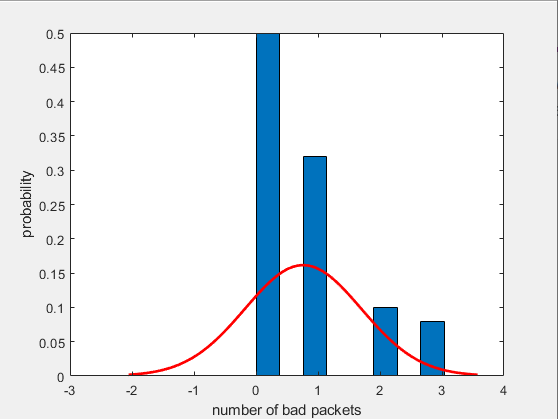
\includegraphics[scale=0.45]{2z5_BSC_005.png}}}
\qquad 
\subfloat[2z5 - kanał REC]{{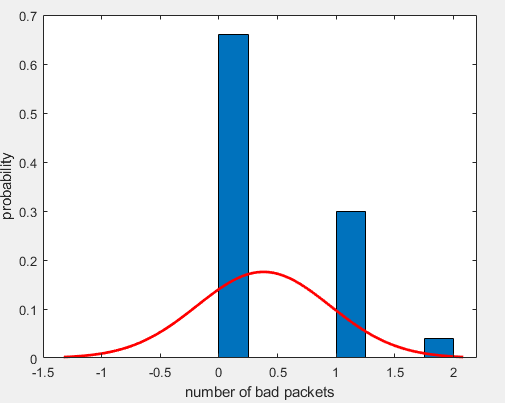
\includegraphics[scale=0.45]{2z5_REC_005.png}}}
\caption{Histogramy dla badanego algorytmu}
\end{figure}

Kod 2 z 5 jest powszechnie stosowany podczas generowania kodów kreskowych, gdzie każda z kresek odpowiada odpowiedniej liczbie zakodowanej w kodzie 2 z 5. Kod ten sprawdza się idealnie, ponieważ pozwala zapisać cyfry z przedziału $<0,9>$. Wykrywalność błędu dla zaimplementowanego kodu wynosi około $70\%$. Dla analizowanych danych, średnia liczba błędów w symulacji jest zbliżona do 0, lecz ilość retransmisji jest znacznie większa niż dla kodu \textit{CRC}. Dla pakietów o większych rozmiarach w kanałach o dużym zaszumieniu przesył danych z użyciem zaproponowanego kodowania może trwać bardzo długo - przesył nie skończy się w racjonalnym czasie. Główną zaletą kodu jest łatwość w implementacji kodera i dekodera, natomiast do głównych wad należy wielkość narzutu dodatkowych bitów przypadających na pakiet, co znacznie wpływa na prędkość oraz czas transmisji. W symulacji pragniemy przesłać informację, która zapisana jest jedynie na $32$ bitach, a w rzeczywistości po zastosowaniu kodu 2 z 5 przesyłamy aż $5 * 32 = 160$ bitów, co odbija się znacząco na czasie przesyłu.

\subsection{Parity bit}

\begin{table}[htbp!]
\begin{tabular}{|c|c|c|c|c|}
\hline
\multicolumn{5}{|c|}{\textbf{Parity bit}}                                                                                  \\ \hline
\textbf{Channel type} & \textbf{Error probability} & \textbf{Packet count} & \textbf{Packet size} & \textbf{Test quantity} \\ \hline
BSC                   & 0.01                       & 10                    & 100                  & 25                     \\ \hline
REC                   & 0.01                       & 10                    & 100                   & 25                     \\ \hline
\end{tabular}
\caption{Zestaw parametrów dla symulacji przeprowadzonej z wykorzystaniem kodu PB}
\end{table}

\begin{table}[htbp!]
\centering
\begin{tabular}{|l|c|c|}
\hline
\diagbox{Parameter}{Canal}& BSC & REC \\ \hline
Mean ($\mu$)                            & 7.44   & 20.72   \\ \hline
Sigma ($\sigma$)                        & 3.4   & 4.68   \\ \hline
Median ($Q_2$)                                          & 7   & 20   \\ \hline
Min ($Q_0$)                                             & 2   & 12   \\ \hline
Max ($Q_4$)                                             & 18   & 34   \\ \hline
IQR ($Q_3-Q_1$)                                          & 4   & 8   \\ \hline
Average number of errors                                 & 8   & 21   \\ \hline
Average transmission length                          & 2 & 2 \\ \hline
Number of additional bits for each packet     & \multicolumn{2}{c|}{1}        \\ \hline
\end{tabular}
\caption{Wykaz parametrów wyznaczonych na podstawie symulacji}
\end{table}

\newpage

\begin{figure}[h!]
\centering
\subfloat[PB - kanał BSC]{{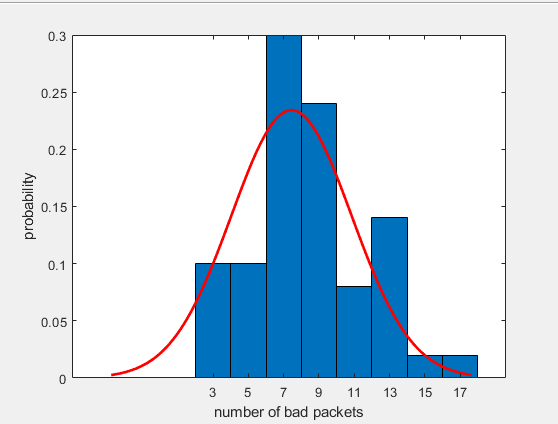
\includegraphics[scale=0.45]{PB_BSC_001.png}}}
\qquad 
\subfloat[PB - kanał REC]{{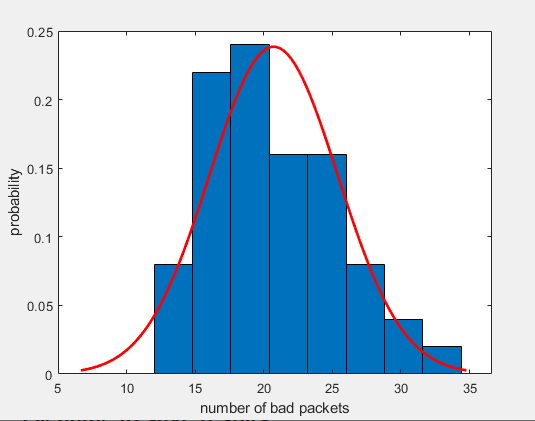
\includegraphics[scale=0.45]{PB_REC_001.png}}}
\caption{Histogramy dla badanego algorytmu}
\end{figure}

Kod polegający na dodaniu bitu parzystości, który równy jest sumie logicznej wszystkich przesyłanych bitów, jest jednym z najprostszych sposobów kontroli poprawności transmitowanych danych. Główną zaletą kodowania jest narzut wyłącznie jednego bitu na przesyłane dane, lecz odbywa się to kosztem dużej liczby błędów podczas transmisji. W porównaniu do poprzednich zaimplementowanych algorytmów, histogram dobrze nakreśla liczbę błędnie przesłanych pakietów. Zgodnie z implementacją kanału \textit{REC} w którym występuje większe zaszumienie niż w kanale \textit{BSC}, występuje tam większa liczba błędów. Główną zaletą stosowanego kodu jest możliwość przesyłania pakietów o dużej liczbie bitów, ponieważ narzut jest znikomy w porównaniu do przysłanej wiadomości lecz transmitowane dane na pewno zawierać będą przekłamania. Kolejną zaletą kodu jest bardzo szybki czas transmisji w kanale oraz łatwość w implementacji kodera i dekodera. Detekcja błędów z użyciem bitu parzystości, może mieć zastosowanie jedynie tam gdzie dopuszczalny jest duży procent błędnie przesłanych pakietów w stosunku do całej transmitowanej informacji.


\subsection{Zestawienie danych ze względu na kanał transmisyjny}

Aby lepiej nakreślić różnice pomiędzy kodowaniami, postanowiliśmy również stworzyć wykresy, które pozwolą na graficzne zobrazowanie liczby występujących błędów oraz retransmisji w zależności od zastosowanego algorytmu i długości przesyłanych pakietów. Taka analiza pozwala na wyznaczenie optymalnych algorytmów dla zadanej długości pakietów oraz kanału transmisyjnego.

Dla każdego z kanałów oraz algorytmów przeprowadziliśmy serię pomiarów w których zmienialiśmy jedynie długość pakietów i notowaliśmy liczbę błędnie przesłanych pakietów wraz z ilością retransmisji przypadającą na pakiet w danej symulacji.

Dla każdej symulacji przyjęliśmy następujące założenia:

\begin{itemize}
    \item Prawdopodobieństwo wystąpienia błędu wynosiło 0.5\%.
    \item Liczba przesyłanych pakietów równa była 20.
    \item Liczba symulacji wynosiła 10.
\end{itemize}

\noindent
Dla każdego zestawu danych uzyskanego z przeprowadzonych symulacji z powyższymi parametrami wyznaczyliśmy średnie wartości z otrzymanych wyników dla każdego z algorytmów w danym kanale. Poniżej zaprezentowano końcowe wyniki w postaci tabelarycznej oraz na wykresach, które podzielone zostały ze względu na kanał transmisyjny.

\newpage

\begin{table}[h!]
\begin{tabular}{|c|c|c|c|c|}
\hline
\textbf{Canal}                 & \textbf{Encoding}             & \textbf{Packet length} & \textbf{Error counter} & \textbf{Transmission length rate} \\ \hline
\multirow{15}{*}{\textbf{BSC}} & \multirow{5}{*}{\textbf{CRC}} & 20                     & 0                      & 1.26                              \\ \cline{3-5} 
                               &                               & 30                     & 0                      & 1.2                               \\ \cline{3-5} 
                               &                               & 40                     & 0                      & 1.27                              \\ \cline{3-5} 
                               &                               & 50                     & 0                      & 1.43                              \\ \cline{3-5} 
                               &                               & 60                     & 0                      & 1.46                              \\ \cline{2-5} 
                               & \multirow{5}{*}{\textbf{2F5}} & 20                     & 0                      & 1.69                              \\ \cline{3-5} 
                               &                               & 30                     & 0                      & 2.17                              \\ \cline{3-5} 
                               &                               & 40                     & 0                      & 2.88                              \\ \cline{3-5} 
                               &                               & 50                     & 0                      & 3.64                              \\ \cline{3-5} 
                               &                               & 60                     & 0                      & 4.26                              \\ \cline{2-5} 
                               & \multirow{5}{*}{\textbf{PB}}  & 20                     & 0.2                    & 1.15                              \\ \cline{3-5} 
                               &                               & 30                     & 0.4                    & 1.15                              \\ \cline{3-5} 
                               &                               & 40                     & 0.6                    & 1.17                              \\ \cline{3-5} 
                               &                               & 50                     & 0.6                    & 1.21                              \\ \cline{3-5} 
                               &                               & 60                     & 1.2                    & 1.37                              \\ \hline
\multirow{15}{*}{\textbf{REC}} & \multirow{5}{*}{\textbf{CRC}} & 20                     & 0                      & 2.13                              \\ \cline{3-5} 
                               &                               & 30                     & 0                      & 2.83                              \\ \cline{3-5} 
                               &                               & 40                     & 0                      & 3.01                              \\ \cline{3-5} 
                               &                               & 50                     & 0                      & 3.79                              \\ \cline{3-5} 
                               &                               & 60                     & 0                      & 4.88                              \\ \cline{2-5} 
                               & \multirow{5}{*}{\textbf{2F5}} & 20                     & 0                      & 8.93                              \\ \cline{3-5} 
                               &                               & 30                     & 0.3                    & 23.74                             \\ \cline{3-5} 
                               &                               & 40                     & 0.7                    & 62.07                             \\ \cline{3-5} 
                               &                               & 50                     & 0.4                    & 197.73                            \\ \cline{3-5} 
                               &                               & 60                     & 0.3                    & 574.77                            \\ \cline{2-5} 
                               & \multirow{5}{*}{\textbf{PB}}  & 20                     & 4.2                    & 1.38                              \\ \cline{3-5} 
                               &                               & 30                     & 8.7                    & 1.59                              \\ \cline{3-5} 
                               &                               & 40                     & 12.8                   & 1.63                              \\ \cline{3-5} 
                               &                               & 50                     & 15.4                   & 1.74                              \\ \cline{3-5} 
                               &                               & 60                     & 24.9                   & 1.79                              \\ \hline
\end{tabular}
\caption{Liczba błędów i ilość transmisji przypadająca na pakiet w danym kanale}
\end{table}

\noindent
Poniżej zamieszczono wykresy utworzone na podstawie danych zamieszczonych w powyższej tabeli. Dla każdego z kanałów wyznaczono zależność liczby błędów oraz transmisji w zależności od długości przesyłanego pakietu.

\begin{figure}[h!]
\centering
\subfloat[Liczba błędnie przesłanych pakietów kanał BSC]{{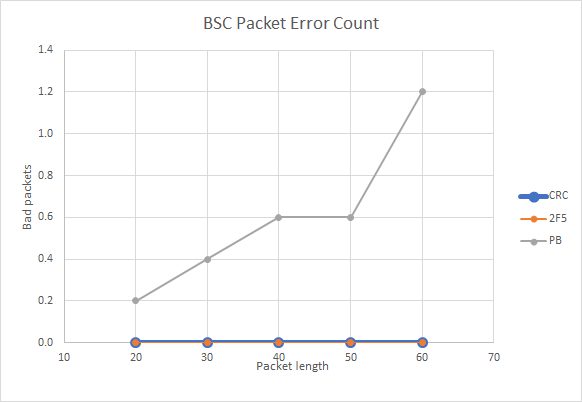
\includegraphics[scale=0.45]{BSC-PEC.png}}}
\qquad 
\subfloat[Liczba błędnie przesłanych pakietów kanał REC]{{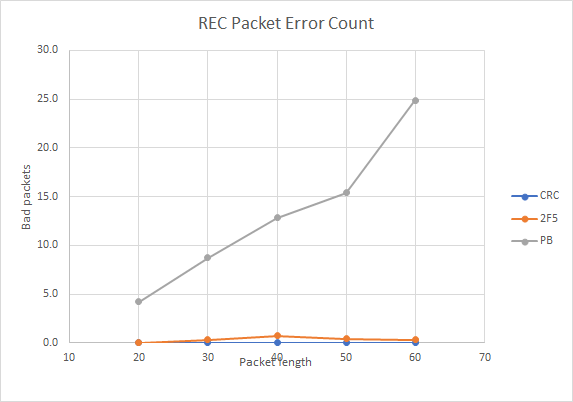
\includegraphics[scale=0.45]{REC-PEC.png}}}
\caption{Zależność ilości błędnie przesłanych pakietów od długości przesłanej informacji}
\end{figure}


\newpage

\noindent
Poniższe wykresy prezentują średnią ilość retransmisji potrzebną na przesłanie jednego pakietu w danym kanale w zależności od długości informacji oraz zastosowanego kodowania.


\begin{figure}[h!]
\centering
\subfloat[Średnia ilość retransmisji kanał BSC]{{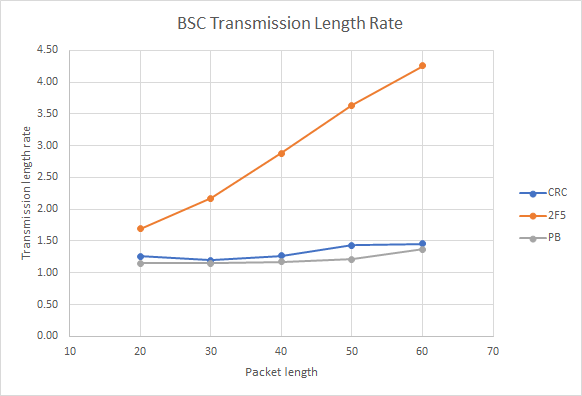
\includegraphics[scale=0.45]{BSC-TLR.png}}}
\qquad 
\subfloat[Średnia ilość retransmisji kanał REC]{{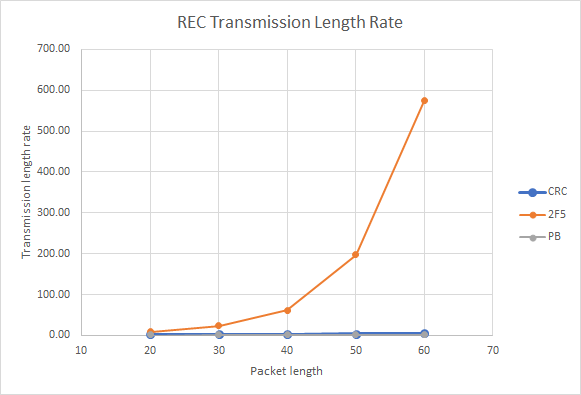
\includegraphics[scale=0.45]{REC-TLR.png}}}
\caption{Zależność średniej ilości retransmisji od długości przesłanej informacji}
\end{figure}

\noindent
Analizując powyższe wykresy widzimy, że wraz ze wzrostem wielkości pakietów kodowanie stosujące bit parzystości nie wykrywa co raz to większej liczby błędnie przesłanych pakietów, natomiast zarówno kodowanie 2z5 jak i \textit{CRC} niewrażliwe są na zmianę długości pakietów. Ponieważ implementacja kanału \textit{REC} charakteryzuje się większym zaszumieniem od kanału \textit{BSC}, liczba błędnych pakietów dla kodowania z wykorzystaniem \textit{PB} jest znacznie większa.

Porównując wykresy dotyczące ilości retransmisji dla każdego z kodowań w zależności od kanału zauważyć możemy znaczący wzrost ilości retransmisji dla kodowania 2 z 5. Spowodowane jest to schematem kodowania, który zamienia każdy z przesyłanych bitów na 5 w związku z czym istnieje większa szansa przekłamania każdego z bitów co przekłada się na ilość retransmisji. Najmniejsza liczba retransmisji, która nie zmienia się dla długości pakietów, zachodzi dla kodowania z wykorzystaniem \textit{PB}, lecz wiąże się to z dużą liczbą błędów podczas transmisji, których stosowany algorytm nie jest w stanie wykryć. Zależność ilości retransmisji dla kodowania 2 z 5 od długości pakietów dla kanału \textit{REC} rośnie wykładniczo i już dla pakietów o długości 50 bitów jeden pakiet transmitowany jest średnio 200 razy co znacznie spowalnia cały przesył sygnału.

Biorąc pod uwagę wszystkie wyciągnięte wcześniej wnioski oraz dane zaprezentowane na wykresach najbardziej optymalnym kodowaniem jest proces wykorzystujący algorytm \textit{CRC}. Wersja szesnastobitowa sprawdza się idealnie dla zadanych długości pakietów, zapewniając 100\% poprawności przesyłanych danych oraz niską liczbę retransmisji, tym samym dodając jedynie narzut 16 bitów do przesyłanego pakietu. Kodowanie 2 z 5 również zapewnia prawie 0\% błędów dla przesyłanej wiadomości lecz ilość retransmisji oraz narzut na przesyłaną informację jest znacząco większy od wartości dla kodowania \textit{CRC}. Natomiast naiwne kodowanie z wykorzystaniem bitu parzystości, nie pozwala na wykrycie wielu błędów podczas transmisji, ale zapewnia stałą liczbę retransmisji niezależną od długości pakietów.

\section{Podsumowanie}

Realizowany temat dobrze nakreślił problem bezbłędnego przesyłu danych w kanale transmisyjnym. Wszystkie z wcześniej założonych celów projektowych zostały poprawnie zrealizowane. Dodatkowo dodaliśmy interfejs graficzny, który w intuicyjny sposób pozwala na przeprowadzanie symulacji dla zadanych parametrów transmisji.

Podczas implementacji mieliśmy okazję dogłębnie poznać oraz analizować model systemu \textit{ARQ}, który poznaliśmy na wcześniejszym semestrze. Wybór środowiska \textit{Matlab} był bardzo trafny, ponieważ dostępne wbudowane funkcje znacznie ułatwiły nam realizację całego projektu, między innymi dostępność funkcji odpowiedzialnej za kodowanie i dekodowanie w algorytmie \textit{CRC} oraz metoda \textit{histfit}, która na podstawie wygenerowanego histogramu pozwalała na uzyskanie odpowiednich danych statystycznych. 

Analiza uzyskanych danych pozwoliła na określenie optymalnych algorytmów dla przesyłanych danych w zależności od długości pakietów oraz kanału w którym przesyłane będą dane.

\newpage

\begin{thebibliography}{9}

\bibitem{Matlab}
Dokumentacja środowiska Matlab
\\\texttt{https://www.mathworks.com/help/matlab/}

\end{thebibliography}

\end{document}
